\documentclass[journal]{IEEEtran}
%\documentclass[journal,draftcls]{IEEEtran}
% Add the compsoc option for Computer Society conferences.
%
% If IEEEtran.cls has not been installed into the LaTeX system files,
% manually specify the path to it like:
% \documentclass[conference]{../sty/IEEEtran}

\usepackage[usenames]{color}
\usepackage{graphicx}
\usepackage{multirow}
\usepackage{caption}
\usepackage{subcaption}
\usepackage{url} 
\usepackage{enumerate}
\usepackage{flushend}

\usepackage{caption}
\usepackage{subcaption}
% DOCUMENT

\usepackage{draftwatermark}                                                                                                  
\begin{document}
%
% paper title
\title{Statement of Purpose}
\author{
\IEEEauthorblockN{Ryan A. Rodriguez}
\IEEEauthorblockA{\\Undergraduate, Department of Electrical Engineering\\UC Santa Cruz, Santa Cruz, CA 95064\\
Email: ryarodri@ucsc.edu, URL: http://www.empireryan.com}
}
\maketitle
\section{Introduction}
At UC Santa Cruz, my coursework has shown me the limits of what is currently possible, and it has convinced me of the fact that a graduate degree is essential for my development as a competent engineer. Although my ultimate goal is to earn a PhD in order to pursue a career in research, a Master of Sciences degree is the right next step for me because it will allow me to make a more informed decision about my particular field of study, and to become a more capable researcher in the interim. To me, a graduate education in engineering is about taking a genuine curiosity, and using that to push the limits of what we know; countless hours of study, and many all-nighters in the lab, the triumphs, but far more numerous failures of these past four years have not deterred my resolve to pursue my goal of having a professional career as a research scientist. 

I'm excited at the prospect of pursuing the MS degree in Computer Engineering at the University of California Santa Cruz, and humbled by this opportunity to deepen my technical knowledge in the field, hone my ability to conduct world-class research, and to push the limits of my profession. As the majority of my peers prepare to accept their comfortable new positions in industry, I write the admissions committee today in the hopes that I can extend my time as a student. 


\section{Background}
\subsection{Project 1 - MEMS}
My first real encounter with a problem demanding exhaustive research was during the spring of my junior year at UC Santa Cruz. I had enrolled in my first graduate course in microelectromechanical systems taught by Dr. Joel Kubby, and the final project was to design a continuous face-sheet deformable mirror to be used for adaptive optics. The design requirements called for micrometer scale actuators that were powerful enough to bend the gold and poly-silicon mirror surface, but stable enough to maintain a linear operation at strokes past two-thirds of the initial electrode gap. 

This problem is difficult because regions beyond this point are typically characterized by instability and non-linearities due to a coulombic pull-in phenomena. A simple fix is to increase the initial gap between electrodes to achieve the desired linear region; however, this was not possible in the multi-user process that we were constrained by. 

After days of sifting through MEMS journals, I stumbled upon a paper that described the use of series capacitance to allow for extended stroke in MEMS actuators. While the electromagnetic theory was ingenious, their folded spring design saw astable performance from asymmetries introduced in the manufacturing process - the result was an actuator that tilted excessively during its descent. Though the authors deemed this problem a fundamental limitation of the technology, I was convinced I had the solution to the instability problem. By using fixed-guided springs in an 'X' pattern, my design would have a stiffer response than the folded springs by forming a negative mechanical feedback loop. 

By integrating trapezoidal capacitors that I'd designed into the spaces left by the the new cross-beam springs, not only did I achieve an extended range of travel, but I minimized the effect of topographical features on the mirrored surface. Ultimately, the research pushed me to develop electrical and mathematical models to optimize my design, and to become adept at using finite element analysis to test my hypotheses. As an undergraduate with a chip on my shoulder in a class full of graduate students, not only did my design achieve the largest stable stroke, but I supported my results with an overwhelming amount of evidence.  

\subsection{Project 2 - Data-Intensive Scientific Workflows}
During the Summer of 2013 I was offered a National Science Foundation grant to work with the Team for Research in Ubiquitous Secure Technology at UC Berkeley. Out of a select group, I was chosen to work on the Tigres project with the Advanced Computing for Science division at Lawrence Berkeley National Laboratory, or LBL, under Dr. Lavanya Ramakrishnan. Tigres is a Python API born of the realization that the vast majority of scientific workflows can be composed from a small set of templates representing common computational patterns, and was designed to streamline the process of writing and executing data-intensive scientific workflows on a wide array of high performance computing resources.

Although research has shown that scientists prefer to code their workflows by hand, almost all modern workflow managers turn to a visual interface. My research during that summer focused on the feasibility and design of an innovative new interface that would allow a scientist's hand-coded workflows to be visualized instantly, and for changes in a visual editor to generate the code needed to execute a given workflow. A third aspect of the interface was a command line tool for code generation that could provide users with the Tigres framework necessary to execute complex workflows with a very minimal syntax. My active console and visual editor offered scientists the flexibility of code while allowing for invaluable visual feedback, and time-saving code generation features available in other workflow tools. 

After a brief hiatus, I spent two quarters performing independent research on the execution engine Tigres uses to run workflows while taking coursework at the prestigious University of Ghana in West Africa. My new research on Tigres focused on data locality, workflow-manager decentralization, and the adaptation of techniques used in MapReduce implementations to data-intensive science on future exascale computers.

I can say for certain that my experience at LBL cemented my decision to pursue advanced study. Being at a place where ideas trump hierarchy, surrounded by some of the smartest people on the planet was truly inspirational, and convinced me that a career in research was the only path for me. 

\subsection{Project 3 - Mechatronic Systems}
The following Fall quarter I enrolled in Dr. Gabriel Elkaim's Introduction to Mechatronics course. The class is notorious for being amongst the most difficult in the department of engineering at UCSC, so naturally I was drawn to the challenge. The course crams Stanford's three quarter long mechatronics design experience into a single quarter where teams of three to five students build a fully autonomous rover capable of navigating an obstacle course while firing ping-pong balls at an opposing robot. 

My experience that quarter was nothing short of transformative because instead of just learning theory, we were expected to make our ideas come to life. Through laser cutting mechanical prototypes, soldering circuits by hand under impossible deadlines, and tying it all together with an embedded system, I learned that one of my most valuable skills is being able to understand, integrate, and troubleshoot complex processes. 

In my spare time, I've been developing a personal mechatronic project for precise sensor and transducer positioning using networked control through asynchronous serial lines. The iteration I'm working on now is intended to be used by recording engineers, and it leverages a cyber-physical system in order to actuate a microphone with three-degrees-of-freedom. Analog input at the control end is packeted with error-control coding of my own design, and sent over balanced transmission lines to a second microcontroller that actuates a set of stepper motors and servos. In addition to honing my skills with embedded systems, this project has given me the opportunity to further develop an optical-potentiometer that has the potential to replace rotary encoders in the feedback loop of certain systems with the added benefit of decreased mechanical complexity, and reduced cost. 

\subsection{Project 4 - Hybrid Inverter}

For my senior design project, I'm working on implementing a hybrid control algorithm for power inverters that has been developed by researchers under the guidance of Professor Ricardo Sanfelice here at UC Santa Cruz. Over the next six months, my team and I will assess the performance of the new algorithm as it compares to traditional implementations that rely on pulse-width modulation. Additionally, we are researching how power conversion on the micro-inverter scale can increase the efficiency of solar networks, and how wide band gap semiconductors can increase power density. With the help of my team, I'll be implementing the boost and inverter hardware, along with the controller for the inverter. 
 
\section{Objectives}

I believe that my research experience aligns closely with work being done by Professor Ricardo Sanfelice at the Hybrid Dynamics and Control group, or HDC, at UC Santa Cruz. At the HDC, pioneering work on cyber-physical systems and control is being done. I strongly believe that my experience with MEMS sensors and actuators, autonomous systems and data-intensive workflow execution, and additionally, my experience with hybrid systems will make me an asset to the group and the department.
It is my hope that this short outline of my work has demonstrated to the admission committee that I have the dedication and aptitude to pursue a graduate education at UC Santa Cruz, and indicated that I have the ability to study problems in diverse areas at a high level.

If I could provide the committee the clearest indication of my commitment to graduate study culminating in a Masters, let it be in my understanding that this will be one of the hardest things that I've ever done, that I'll work long hours solving problems so that more difficult problems can take their place, and that I'll do it for less pay than my peers in industry - and in spite of these realizations, I write you today asking wholeheartedly for admission. 
The interdisciplinary nature of research in cyber-physical systems is perhaps the most challenging, but surely the most exciting aspect of pursuing a Masters degree in this field. It is my sincerest hope that I can pursue my goal of becoming a research scientist by continuing my coursework and research at UC Santa Cruz.

\begin{IEEEbiography}[{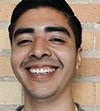
\includegraphics[width=1 in,height=1 in, clip, keepaspectratio]{./RodriguezR}}]{Ryan Rodriguez} 
was born in 1989 and completed his elementary and secondary education in the East Bay Area. He is a graduate of the USAF's ground radio and satellite communication school at Keesler AFB in Biloxi, MS where he also earned an FBI level 'Secret' security clearance. Ryan is currently completing the final year of his BS in Electrical Engineering at UC Santa Cruz, and finishing his senior design and research cycle. Ryan is interested in MEMS, mechatronics, embedded and cyber-physical systems, control, the economics of information, entrepreneurship and law. 
\end{IEEEbiography}

\end{document}
